\documentclass[12pt,twoside]{article}
\usepackage{amsmath, amssymb}
\usepackage{amsmath}
\usepackage[active]{srcltx}
\usepackage{amssymb}
\usepackage{amscd}
\usepackage{makeidx}
\usepackage{float}
\usepackage{amsthm}
\usepackage{algpseudocode}
\usepackage{algorithm}
\usepackage{graphicx}
\usepackage[spanish, es-tabla]{babel}
\usepackage{multirow}
\usepackage{cite}
\renewcommand{\baselinestretch}{1}
\graphicspath{{images/}}
\setcounter{page}{1}
\setlength{\textheight}{21.6cm}
\setlength{\textwidth}{14cm}
\setlength{\oddsidemargin}{1cm}
\setlength{\evensidemargin}{1cm}
\pagestyle{myheadings}
\thispagestyle{empty}
\markboth{\small{Pr\'actica 8. Alan, Josu\'e}}{\small{.}}
\date{}
\begin{document}
\centerline{\bf An\'alisis de Algoritmos, Sem: 2020-1, 3CV2, Pr\'actica 8, 2 de octubre}
\centerline{}
\centerline{}
\begin{center}
\Large{\textsc{Pr\'actica 8: Multiplicaci\'on de una secuencia de matrices}}
\end{center}
\centerline{\bf{Alan Romero Lucero, Josu\'e David Hern\'andez Ram\'irez}}
\centerline{}
\centerline{Escuela Superior de C\'omputo}
\centerline{Instituto Polit\'ecnico Nacional, M\'exico}
\centerline{$alanrl.escom@gmail.com, josuehernandezr082@gmail.com$}
\newtheorem{Theorem}{\quad Theorem}[section]
\newtheorem{Definition}[Theorem]{\quad Definition}
\newtheorem{Corollary}[Theorem]{\quad Corollary}
\newtheorem{Lemma}[Theorem]{\quad Lemma}
\newtheorem{Example}[Theorem]{\quad Example}
\bigskip
\textbf{Resumen:} El presente documento desarrolla la implementaci\'on de un algoritmo para la multiplicaci\'on de una secuencia de matrices, aplicando el concepto de programaci\'on din\'amica..{\bf Palabras Clave:} {\textit{matrices, producto matricial, programaci\'on din\'amica, configuraci\'on \'optima.}}
\section{Introducci\'on}
Existen problemas que encuentran una soluci\'on \'optima mediante algoritmos recursivos, los cuales logran tener una complejidad bastante \textit{aceptable}, sin embargo, algunos otros problemas a pesar de tener una buena complejidad pueden ser optimizados mediante otros tipos de algoritmos o pr\'acticas de programaci\'on, como lo es la programaci\'on dinamica. La programaci\'on dinamica es principalmente una optimizaci\'on para algoritmos generalmente recursivos, donde se almacenan configuraciones \'optimas para el algoritmo, de manera que no se tengan que computar por cada ciclo o se pueda decidir entre las configuraciones por la que represente menor complejidad. Por esto se aplicar\'a la programaci\'on dinamica para resolver el problema de \textit{\textbf{multiplicaci\'on de una secuencia de matrices}}.

El problema de la \textit{multplicaci\'on de una secuencia de matrices} no es el del producto entre matrices per se, desde que se puede utilizar el algoritmo de strassen o el algoritmo usual para la multiplicaci\'on de matrices. El problema es buscar la configuraci\'on \'optima de par\'entesis, llamada a partir de ahora \textit{parentizaci\'on}, que agrupara la secuencia de matrices de manera tal que se realizar\'an la menor cantidad de productos escalares.

\section{Conceptos B\'asicos}
\subsection{Empezando con la programaci\'on din\'amica}
Para aplicar la programaci\'on din\'amica a un problema para su optimizaci\'on se deben seguir los siguientes \textit{pasos}:

\begin{itemize}
    \item \textbf{Caractersizaci\'on de la estructura de una soluci\'on \'optima.} Se analiza el problema buscando la estructura que deber\'ia tener la soluci\'on \'optima al problema.
    \item \textbf{Una soluc\'on recursiva.} Una vez identificada la estructura de la soluc\'on \'optima, se plantea la misma como una funci\'on recursiva, dado que el problema puede ser dividido subproblemas que se pueden llevar a su vez a una estructura \'optima.
    \item \textbf{Computando el costo \'optimo.} Una vez identificada la funci\'on recursiva que describe la estructura de una soluc\'on \'optima, se computan los costos \'optimos y se van almacenando.
    \item \textbf{Construir la soluci\'on con el costo \'optimo computado.} Finalmente se da la soluc\'on al problema basado en los costos \'optimos previamente computados, los cuales fueron almacenados.
\end{itemize}

Es importante destacar que, debido a las caracter\'isticas de la programaci\'on din\'amica, su complejidad computacional no deber\'ia solo considerar el tiempo de ejecuci\'on, sino tambi\'en el \textit{consumo de recursos que representa} su implementaci\'on.

\subsubsection{Aplicaci\'on de conceptos al problema}

Entonces, dado el problema de la \textit{multplicaci\'on de una secuencia de matrices} se busca la estructura de soluci\'on \'optima. 

Se tiene $A_{i\dots j}$ como la matriz solucion al producto de las matrices $A_i \dots A_j$ con la configuraci\'on. Adem\'as se sabe que la matriz $A_{i \dots j}$ debe ser el producto de otras dos matrices, las cuales se pueden escribir como $A_{i \dots k}$ y $A_{k+1 \dots j}$ donde $i \leq k \leq j$; estas matrices son el producto de $A_i A_{i+1} \dots A_{k-1} A_k$ y $A_{k + 1} A_{k+2} \dots A_{j-1} A_j$, respectivamente.

Como la matriz $A_{i\dots j}$ tiene una parentizaci\'on \'optima, se puede asegurar que  $A_{i \dots k}$ y $A_{k+1 \dots j}$ tambi\'en son la soluciones \'optimas. Si alguna de las dos matrices no tuviera una parentizaci\'on \'optima, significar\'ia que existe alguna otra parentizaci\'on que lo es; dado que existe otra configuraci\'on \'optima diferente ya sea para  $A_{i \dots k}$ o $A_{k+1 \dots j}$ no se puede afirmar que la parentizaci\'on de $A_{i\dots j}$ sea \'optima, entrando en una contradicci\'on.

Ahora, se tiene $m[i][j]$, que representa el costo o n\'umero de productos escalares \'optimo del producto matricial para la matriz resultante $A_{i \dots j}$. Adem\'as se considera que el n\'umero de productos escalares entre las matrices $A_i \times A_{i+1}$ son $p[i-1] \times p_i \times p_{i+1}$. Entonces, dada la estructura de soluci\'on \'optima planteada anteriormente, el costo $m[i][j]$ se calcula con el costo \'optimo de las matrices $m[i][k]$ y $m[k+1][j]$, y el n\'umero de productos escalares $p_i-1 \times p_k \times p_j$. Finalmente, el costo para el producto de una sola matriz, es decir, $m[i][i]$, es $0$. Entonces, se tiene la siguiente funcion:
\[
    m[i][j] =
    \begin{cases}
        0 & i = j \\
        min_{i \leq k \leq j}{ m[i][k] + m[k+1][j] + (p_{i-1})(p_k)(p_j) } & i < j
    \end{cases}
\]

Ya que $k$ pertenece al intervalo $[i,j]$ se tomaran el costo minimo entre todos su valores posibles.

Ahora bien, para copmutar los costos optimos el algoritmo es el siguiente.

\begin{figure}[ht]
    \centering
    \begin{algorithmic}
        \Procedure{maxchainmult}{$p = [p_1, \dots, p_n]$}
            \State $m \longleftarrow [n+1][n+1]$
            \State $s \longleftarrow [n+1][n+1]$
            \State // Los indices [0] no se utilizaran por comodidad de la notaci\'on
            \For{$L$ from $2$ to $n$}
                \For{$L$ from $1$ to $n - L + 1$}
                    \State $j \longleftarrow i + L - 1$
                    \State $m[i][j] \longleftarrow 10^{100}$
                    \For{$k$ from $i$ to $j$}
                        \State $q \longleftarrow m[i][k] + m[k+1][j] + (p_{i-1} \times p_k \times p_j)$
                        \If{$q < m[i][j]$}
                            \State $m[i][j] \longleftarrow q$
                            \State $s[i][j] \longleftarrow k$
                        \EndIf
                    \EndFor
                \EndFor
            \EndFor
            \State \textit{\textbf{return}} $m,s$
        \EndProcedure
    \end{algorithmic}
    \caption{Algoritmo para computar todos lo costos optimos para todas las posibles parentizaci\'ones.}
    \label{fig:computo_costos}
\end{figure}

La matriz $s$ va almacenando el indice $k$ por el que se divide la secuencia de matrices de la manera m\'as \'optima, y esto se puede decidir gracias a que los menores costros se almacenan el ma matriz $m$.

Finalmente, una vez computados los menores costos, y los indices que ya est\'an almacenados en la matriz $s$, se da la soluci\'on al problema imprimiendo la parentizaci\'on m\'as \'optima. Esto se hace con el siguiente algoritmo recursivo, adem\'as cuando se ejecuta, se le pasan como parametros la matriz $s$ previamente computadao, 1 y $n$ como el n\'umero de matrices que se multiplicar\'an.

\begin{figure}[ht]
    \centering
    \begin{algorithmic}
        \Procedure{OptimalP}{s[n][n], i, j}
            \If{i=j}
                \State \textit{\textbf{print}} $A_i$
            \Else
                \State \textit{\textbf{print}} (
                \State \textit{\textbf{OPTIMALP}}(s, i, s[i][j])
                \State \textit{\textbf{OPTIMALP}}(s, s[i][j] + 1, j)
                \State \textit{\textbf{print}} )
            \EndIf
        \EndProcedure
    \end{algorithmic}
    \caption{Caption}
    \label{fig:my_label}
\end{figure}

\subsection{¿La fuerza bruta es una opci\'on?}

La parentizaci\'on \'optima tambi\'en puede ser obtenida mediante fuerza bruta, probando todas las configuraciones de parentessis posibles, sin embargo es poco viable. Se usar\'a como notaci\'on para referirse al n\'umero de parentizaci\'ones de $n$ matrices como $P(n)$.
\begin{align*}
    \text{Para } n=1 \longrightarrow P(1) = 1
\end{align*}
\begin{align*}
    \text{Para } n=2 \longrightarrow P(2) = 1 = P(1)P(1)
\end{align*}
\begin{align*}
    \text{Para } n=3 \longrightarrow P(3) = 2 = P(2)P(1) + P(1)P(2) 
\end{align*}
\begin{align*}
    \text{Para } n=4 \longrightarrow P(4) = 5 = P(1)P(3) + P(2)P(2) + P(3)P(1)
\end{align*}
\begin{align*}
    \text{Para } n=5 \longrightarrow P(5) = 14 = P(1)P(4) + P(2)P(3) + P(3)P(2) + P(4)P(1)
\end{align*}

Se puede expresar como la siguiente ecuaci\'on de recurrencia:

\begin{figure}[ht]
    \centering
    \[
        P(n)
        \begin{cases}
            1 & n=1 \\
            \sum_{k=1}^{n-1} P(k)P(n-k) & n>1
        \end{cases}
    \]
    \caption{Ecuaci\'on de recurrencia para el n\'umero de parentizaciones para n matrices}
    \label{eq:recurrencia_p}
\end{figure}

\newpage
\vfill
\clearpage

\section{Experimentaci\'on y Resultados}
\subsection{Ejemplos}
\begin{figure}[ht]
    \centering
    \begin{equation*}
        \text{Para } n=4
    \end{equation*}
    \begin{equation*}
        \text{\textbf{Entrada }} 5,7,2,6,9
    \end{equation*}
    \begin{equation*}
        \text{\textbf{Salida }}
    \end{equation*}
    \begin{equation*}
        \text{\textbf{Configuraciones posibles}}
    \end{equation*}
    \begin{equation*}
        (A_1(A_2(A_3A_4))) \text{  Productos escalares: } 549 
    \end{equation*}
    \begin{equation*}
        (A_1((A_2A_3)A_4)) \text{  Productos escalares: }777
    \end{equation*}
    \begin{equation*}
        ((A_1(A_2A_3))A_4) \text{  Productos escalares: }564
    \end{equation*}
    \begin{equation*}
        (((A_1A_2)A_3)A_4) \text{  Productos escalares: }400
    \end{equation*}
    \begin{equation*}
        ((A_1A_2)(A_3A_4)) \text{  Productos escalares: }268
    \end{equation*}
    \caption{Primer caso de ejemplo de parentizaci\'on}
    \label{eq:primer_ejemplo}
\end{figure}

En la figura \ref{eq:primer_ejemplo}, la configuracion $((A_1A_2)(A_3A_4))$ es la configuraci\'on \'optima, debido a que tiene el menor n\'umero de operaciones escalares. Sin embargo, pese a tener el mismo $n=4$, se encuentra como la soluci\'on m\'as \'optima a la configuraci\'on $(A_1((A_2A_3)A_4))$ en la figura \ref{eq:segundo_ejemplo}.

\begin{figure}[ht]
    \centering
    \begin{equation*}
        \text{Para } n=4
    \end{equation*}
    \begin{equation*}
        \text{\textbf{Entrada }} 23,12,31,11,10
    \end{equation*}
    \begin{equation*}
        \text{\textbf{Salida }}
    \end{equation*}
    \begin{equation*}
        \text{\textbf{Configuraciones posibles}}
    \end{equation*}
    \begin{equation*}
        (A_1(A_2(A_3A_4))) \text{  Productos escalares: } 9890 
    \end{equation*}
    \begin{equation*}
        (A_1((A_2A_3)A_4)) \text{  Productos escalares: }8172
    \end{equation*}
    \begin{equation*}
        ((A_1(A_2A_3))A_4) \text{  Productos escalares: }14465
    \end{equation*}
    \begin{equation*}
        (((A_1A_2)A_3)A_4) \text{  Productos escalares: }18929
    \end{equation*}
    \begin{equation*}
        ((A_1A_2)(A_3A_4)) \text{  Productos escalares: }11966
    \end{equation*}
    \caption{Segundo caso de ejemplo de parentizaci\'on}
    \label{eq:segundo_ejemplo}
\end{figure}

\newpage
\vfill
\clearpage

\subsection{Implementacion}

\begin{figure}[ht]
    \centering
    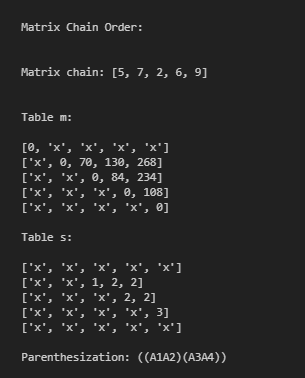
\includegraphics{1.png}
    \caption{Configuracion \'optima del ejemplo \ref{eq:primer_ejemplo}}
    \label{fig:programa_primer}
\end{figure}

\begin{figure}[ht]
    \centering
    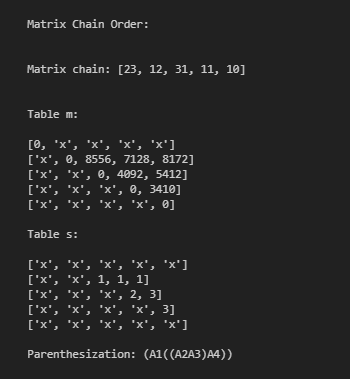
\includegraphics{2.png}
    \caption{Configuracion \'optima del ejemplo \ref{eq:segundo_ejemplo}}
    \label{fig:programa_segundo}
\end{figure}
\newline \newline
Como hemos podido observar en las im\'agenes en donde se demuestra el resultado de la implementaci\'on del algoritmo, se corrobora que, los c\'alculos te\óricos son correctos.
\newpage
\vfill
\clearpage

\section{Conclusiones}

\textit{Alan Romero Lucero}. La programaci\'on din\'amica es tediosa y requiere de un gran an\'alisis y entendimiento del problema para poder aplicarlo efectivamente, como se puede ver en el desarrollo de esta pr\'actica. A pesar de eso, resulta ser una gran solucion a problemas que ya son dificiles de optimizar. Me parece interesante como se van a almacenando los resultado \'optimos y de esta manera se puede reducir la complejidad, ya que solo se tienen que computar una vez. El \'unico inconveniente que le encuentro es que se debe considerar el consumo de recursos que se tendr\'a. Sus aplicaciones pueden ser muchismias, pero realmente encuentro dificil el an\'alisis necesario para poder encontrar la estructura de la soluci\'on \'optima.


\textit{Josu\'e David Hern\'andez Ram\'irez}.
Es el primer programa de algoritmo dinámico que he visto en toda mi carrera informática. Es muy interesante ver que si tenemos una cadena de matrices, dependiendo de cómo nos asociemos para multiplicarlas, resultará en una configuraci\'on \'optima o no. La programaci\'on dinámica funciona particularmente bien para problemas de optimizaci\'on con ordenamiento inherente de izquierda a derecha entre elementos. El \'optimo global resultante a menudo es mucho mejor que la soluci\'on encontrada con la heur\'istica. Y una vez entendida, la programaci\'on din\'amica suele ser más f\'acil de trabajar desde cero que buscar algoritmo.

\section{Anexo}

Recordando la ecuaci\'on de recurrencia:
\[
    P(n)
    \begin{cases}
        1 & n=1 \\
        \sum_{k=1}^{n-1} P(k)P(n-k) & n>1
    \end{cases}
\]

Que adem\'as, genera los n\'umeros de Catalan.

\[
    \text{Supongase que } P(n) \geq c2^k, k > n \text{ entonces } \dots 
\]
\[
    P(n) = \sum_{k=1}^{n-1} P(k)P(n-k) \geq \sum_{k=1}^{n-1} c2^k \times c2^{n-k} 
\]
\[
    \geq \sum_{k=1}^{n-1} c^22^{n}
\]
\[
    \geq (n-1) c^22^{n}
\]
\[
    \sum_{k=1}^{n-1} P(k)P(n-k) \geq c2^{n}
\]
\[
    \exists n_0,c > 0 \text{ que cumplen la condici\'on?}
\]
\[
    n_0 = 5 \longrightarrow P(n = 5) = 42, 2^5 = 32
\]
\[
    42 \geq c32
\]

Con $n_0 = 4$ y $c = \frac{42}{32}$ se cumple la desigualdad, por lo que, segun la definicion de $ \omega $ , $P(n)$ es $\Omega(2^n)$.


\section{Bibliograf\'ia}
[ 1 ] Baase and Van Gelder. ”Computer Algorithms: Introduction to Design and Analysis”. Addison-Wesley.

[ 2 ] Thomas H. Cormen. ”Introduction to Algorithms”. The MIT press.


\end{document}